\documentclass[9pt,a4paper,twoside]{tau}
\usepackage[english, italian]{babel}
\usepackage{tauenvs}

\usepackage{algorithm}
\usepackage{algpseudocode}

\usepackage{listings}


%----------------------------------------------------------
% TITLE
%----------------------------------------------------------

\title{Lighting and Shading: il modello del Ray Tracing}

%----------------------------------------------------------
% AUTHORS, AFFILIATIONS AND PROFESSOR
%----------------------------------------------------------

\author{Antonio Sirignano}

%----------------------------------------------------------

%\affil[a]{Affiliation of author one}
%\affil[b]{Affiliation of author two}
%\affil[c]{Affiliation of author three}

\professor{Calcolo Scientifico per l'Innovazione Tecnologica - prof. Luisa D'Amore}

%----------------------------------------------------------
% FOOTER INFORMATION
%----------------------------------------------------------

\institution{Università degli Studi di Napoli Federico II}
\ftitle{Lighting and Shading: il modello del Ray Tracing}
\date{a.a. 2023-2024}
\etal{Sirignano}
\course{Calcolo Scientifico per l'Innovazione Tecnologica}

%----------------------------------------------------------
% ABSTRACT
%----------------------------------------------------------

\begin{abstract}    
    In questo progetto viene fatta un'introduzione generale al lighting e allo shading, con una presentazione dei modelli di riflessione e di shading che possono essere applicati alla grafica computazionale.\\
    Nel seguito viene presentato in maniera più approfondita il modello del Ray Tracing, con le sue applicazioni, in particolare al mondo del video game e il 3D video editing.
\end{abstract}

%----------------------------------------------------------

\keywords{calcolo scientifico, lighting, shading, ray tracing.}

%----------------------------------------------------------

\begin{document}
		
	\maketitle
	\thispagestyle{firststyle}
	\tauabstract
	\tableofcontents

%----------------------------------------------------------

\section{Introduzione}

    \taustart{L}a Computer Graphic Technology è l'abilità d produrre un effetto visivo realistico in un oggetto tridimensionale in un device di output bidimensionale, come un computer o un foglio stampato.\\
    Tutto ciò si ha grazie ai \textit{metodi di rendering} nei quali è applicato lo \textit{shading} per raggiungere il più possibile una rappresentazione di un oggetto vicina alla realtà.\\ 
    Infatti lo shading computa quantità e colore della luce emessa da ogni punto della superficie.\\
    Tali risultati dipendono dalle seguenti entità:
    \begin{enumerate}
    	\item \textbf{La sorgente di luce}. Intensità, colore, forma, direzione e distanza della sorgente di luce devono essere prese in considerazione e inoltre possono essere sia puntiformi che di grandi dimensioni.
    	\item \textbf{La superficie dell'oggetto}. L'oggetto può essere lucido, liscio, ruvido, brillante o scuro. Può inoltre avere colori differenti quali opachi, trasparenti o traslucidi. 
    	\item \textbf{L'ambiente}. Oggetti visti in uno spazio vuoto, senza un background che rifletta la luce su di essi, risultano duri (una navicella spaziale nello spazio profondo). Un modello realistico di shading deve tenere in considerazione la luce riflessa dagli altri oggetti (pareti vicine).
    \end{enumerate}

\section{Le sorgenti di luce}
\taustart{U}n oggetto illuminato dalla luce è colpito da raggi luminosi proiettati sulla sua superficie da un emittente chiamato \textit{sorgente di luce}. La luce può descrivere diverse scene presentate di seguito.
\begin{enumerate}
    	\item \textbf{Luce ambientale}. Questa luce è una sorgente di luce non direzione la cui luce è emessa da ogni direzione. La sua intensità è indipendente da tutte le sue caratteristiche, come posizione e orientamento.
    		\begin{figure}[H]
        		\centering
       			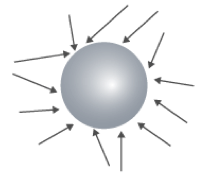
\includegraphics[width=0.6\columnwidth]{Figures/01.png}
       	 		\caption{Luce ambientale}
        		\label{fig:figure}
			\end{figure}
		
    	\item \textbf{Luce puntiforme}. \'E una sorgente di luce che non emette la stessa quantità di luce proveniente da tutte le direzioni, infatti un oggetto quanto è più vicino ad essa tanto è più luminoso. L'intensità della sorgente è quindi dipendente dalla distanza e dalla angolazione. \'E caratterizzata da colore, intensità, posizione e funzione di decadimento.
    		\begin{figure}[H]
        		\centering
        		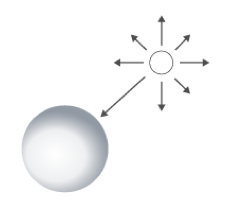
\includegraphics[width=0.6\columnwidth]{Figures/02.png}
        		\caption{Luce puntiforme}
       			\label{fig:figure}
			\end{figure}   
    	
    	\item \textbf{Luce direzionale}. Tale tipo è prodotta da una sorgente di luce da una distanza infinita dalla scena. Tutti i raggi di luce si espandano in una singola direzione e con la stessa intensità ovunque. \'E caratterizzata da colore, intensità e direzione.
    		\begin{figure}[H]
        		\centering
        		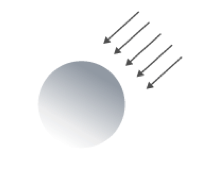
\includegraphics[width=0.6\columnwidth]{Figures/03.png}
        		\caption{Luce direzionale}
        		\label{fig:figure}
			\end{figure}
    	\item \textbf{Spotlight}. La luce si irradia in un cono con più luce al centro di esso. Questa luce è fissata all'asse primario di direzione con una restrizione su di essa. \'E caratterizzata come un punto di propagazione, un asse di direzione, un raggio intorno all'asse e la possibilità di una funzione di decadimento radiale. 
    		\begin{figure}[H]
		        \centering
		        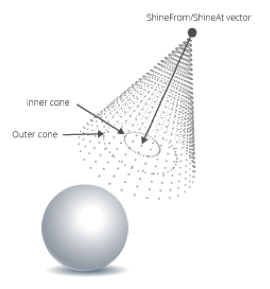
\includegraphics[width=0.6\columnwidth]{Figures/04.png}
		        \caption{Spotlight}
		        \label{fig:figure}
			\end{figure}
\end{enumerate}

\section{Modelli di riflessione}
\taustart{L'}obiettivo principale dello shading è la produzione di un risultato accettabile quando la superficie dell'oggetto è affetta dai raggi di luce. I modelli di riflessione sono presentati di seguito.
\begin{enumerate}
	\item \textbf{Riflessione diffusa}. Tale modello di riflessione diffonde la luce uniformemente in tutte le direzioni. In accordo con la legge di Lambert si ha che la diffusione del riflesso è proporzionale al coseno dell'angolo $\theta$ compreso tra la normale $N$ e la direzione della sorgente $L$. 
		\begin{figure}[H]
	        \centering
	        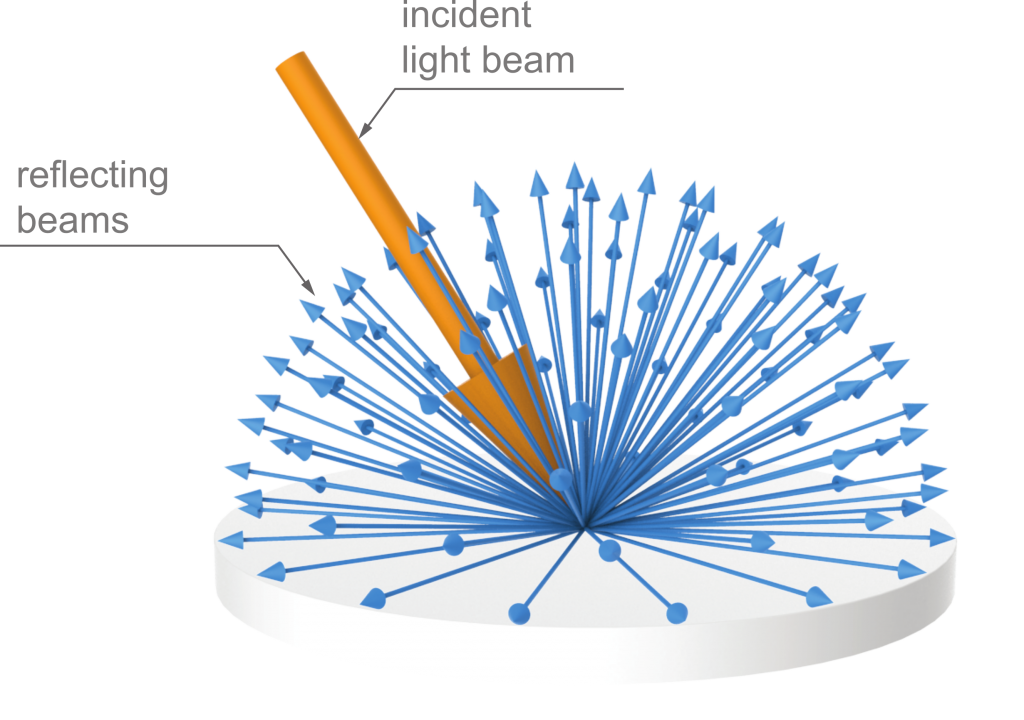
\includegraphics[width=0.6\columnwidth]{Figures/05.png}
	        \caption{Riflessione diffusa}
	        \label{fig:figure}
		\end{figure}
		Da qui
		\begin{equation*}
			\cos{\theta} = L \cdot N
		\end{equation*}
		E considerando il coefficiente di riflessione $k_d$, con $0\leq k_d \leq 1$, si ha
		\begin{equation*}
			R_d = k_d \cdot L \cdot N
		\end{equation*}
		Volendo considerare l'attenuazione della luce, si deve far riferimento alla distanze che essa percorre $d$. Quindi il termine di attenuazione quadratico è
		\begin{equation*}
			R_d = \frac{k_d}{A + BD + C(D \cdot D)}(L \cdot N)
		\end{equation*}
		E quindi
		\begin{equation*}
			I_d = \frac{k_d}{A + AD + A(D\cdot D)}(L \cdot N)
		\end{equation*}
	\item \textbf{Riflessione speculare}. Tale modello produce una riflessione luminosa sulla superficie dell'oggetto.
		\begin{figure}[H]
	        \centering
	        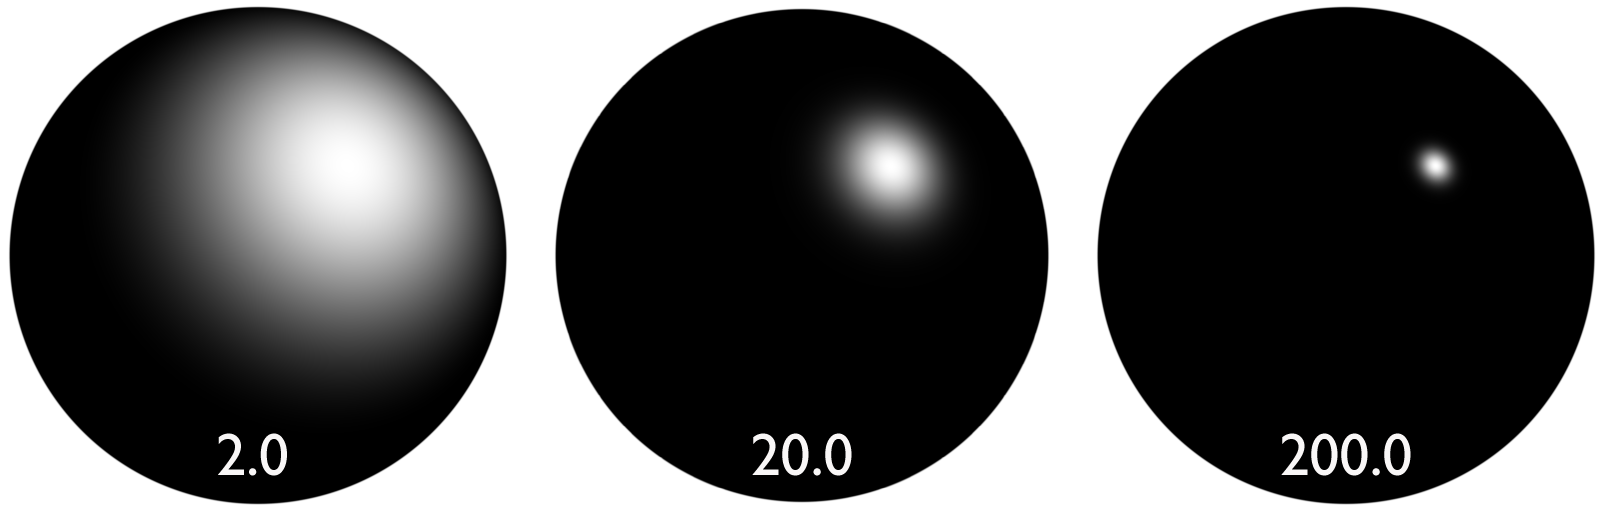
\includegraphics[width=0.6\columnwidth]{Figures/06.png}
	        \caption{Riflessione speculare}
	        \label{fig:figure}
		\end{figure} 
		L'angolo $\phi$ compreso tra la direzione della riflessione $r$ e la direzione $\nu$ dell'osservatore è affetto da una quantità di luce speculare. Il modello Phong stabilisce
		\begin{equation*}
			R_s = k_s \cos{^n}{\phi}
		\end{equation*}
		per coefficiente $k_s$, con $0 \leq k \leq 1$. L'esponente $n$ è il coefficiente di lucentezza. All'incrementare di $n$, la luce riflessa si concentra in una regione superficiale più piccola, centrata in $r$. Valori tra il 100 e il 500 corrispondono a superfici metalliche, valori più piccoli corrispondono a ad illuminazioni più ampie. Quindi
		\begin{equation*}
			R_s = k_s(r \cdot \nu )^n
		\end{equation*}
		Una distanza viene moltiplicata similmente alle riflessioni diffuse.\\
		La combinazione di tre tipi di riflessione danno
		\begin{equation*}
			I=\frac{1}{A + BD + C(D \cdot D)}(K_d(L \cdot N)L_d + k_s(r \cdot \nu)nL_s) + K_aL_a
		\end{equation*}
		La direzione della riflessione $r$ è semplice da $n$ e $I$, assumendo che $n$ sia un'unità di lunghezza, inoltre si vede che
		\begin{equation*}
			\frac{L+r}{2}=(L \cdot n)n \implies r = 2(L \cdot n)n - L
		\end{equation*}
\end{enumerate}

\section{Modelli di shading}
\taustart{I} modelli di shading sono utilizzati per ottenere il modello di illuminazione desiderato. Modelli di shading efficienti per la superficie definita da un poligono si possono descrivere come seguono.
\begin{enumerate}
	\item \textbf{Constant shading}. Questo modello è il più semplice modello di shading anche conosciuto come faceted shading o flat shading. Lo stesso colore è applicato su ogni intero poligono con un rendering veloce. L'equità della luce è usata una sola volta per poligono. Data una singola normale al piano, l'equazione della luce e le proprietà del materiale sono usate per generare un singolo colore. Il poligono avrà tale colore.
		
	\item \textbf{Gouraud shading}. Questo modello è anche chiamato intensity interpolation shading o color interpolation shading. I colori sono interpolati attraverso il poligono e vi è la necessità di identificare ogni vertice. Il processo di rendering è più lento rispetto al modello flat. L'equità della luce è applicata ad ogni vertice e anche ogni colore è determinato dalla quantità di luce con le proprietà del materiale. La Scan-line interpolation è usata per assegnare un colore ad ogni punto di proiezione del poligono come la media pesata dei colori di dati vertici.
	\item \textbf{Phong shading}. Tale modello è più realistico degli altri perché il suo algoritmo considera l'unione delle normali dei vertici ad ogni punto del poligono per avere una normale locale. Inoltre, il calcolo è applicato per avere un'illuminazione totale nel rendering.
\end{enumerate}
\begin{figure}[H]
    \centering
    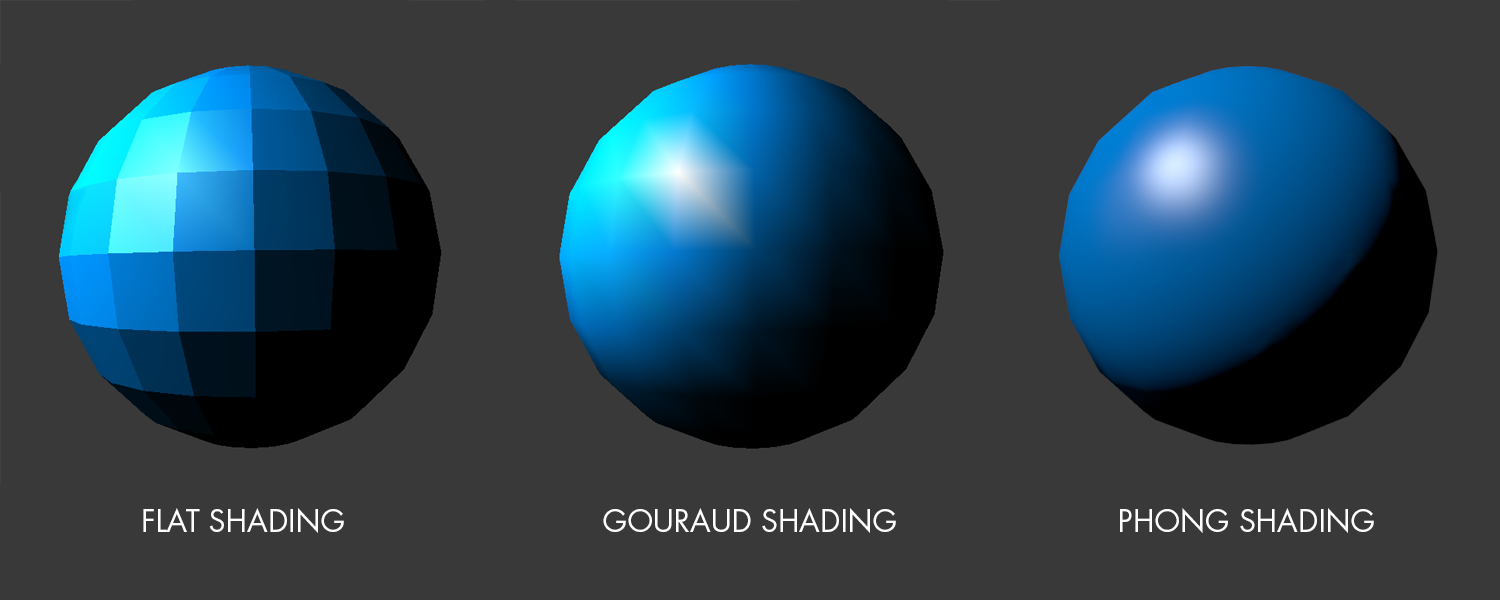
\includegraphics[width=0.7\columnwidth]{Figures/07.png}
    \caption{Flat, Gouraud e Phong shading}
    \label{fig:figure}
\end{figure}	

\section{Il modello del Ray Tracing}
\taustart{L'}ambizione degli artisti, dei designers, degli ingegneri è sempre stata la simulazione dell'immagine di una scena, una storia, un prodotto, un palazzo prima che sia effettivamente realizzati e costruiti - architetti devono costruire modelli in scala, produttori di film e video-game devono utilizzare storyboards per provare e trasmettere le sensazioni di un film o un video-game. E gli inserzionisti vogliono creare interpretazioni perfette dei loro prodotti nella migliore luce possibile. Inoltre i designer di prodotti e macchinari vogliono trovare le debolezze di un progetto prima che esso venga effettivamente costruito - direttori di film vogliono vedere il risultato finale prima dell'arduo lavoro di post-produzione, i produttori vogliono mostrare a potenziali clienti il prodotto finale per stimolarne la domanda. Il test di tali idee è chiamato virtual prototyping nella manifattura e pre-visualization nell'industria cinematografica. Vi è quindi la necessità di disporre di queste immagini, o video, a basso costo e in poco tempo.\\

\section{L'equazione di rendering}
\taustart{N}ella computer graphics, l'equazione di rendering è un'equazione integrale nella quale la radianza di equilibrio che lascia un punto è la somma della radianza emessa più la radianza riflessa sotto un'approssimazione dell'ottica geometrica.
\begin{figure}[H]
    \centering
    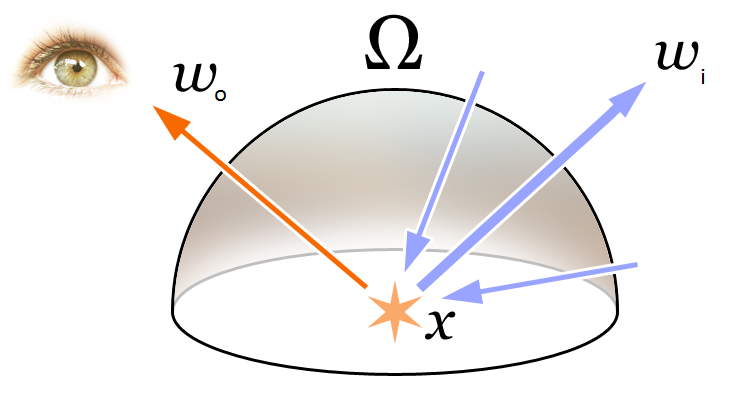
\includegraphics[width=0.7\columnwidth]{Figures/08.png}
    \caption{Equazione di rendering}
    \label{fig:figure}
\end{figure}
Esistono svariate tecniche di rendering nella computer graphics che cercano di risolvere tale equazione.
L'equazione di rendering descrive la quantità totale di luce emessa da un punto $x$ lungo una particolare direzione di osservazione, data una funzione per la luce in entrata e una funzione di distribuzione bidirezionale di riflettenza (BRDF), dove,
\begin{itemize}
	\item $x$ è una posizione nello spazio
	\item $w_o$ è la direzione della luce in uscita
	\item $\Omega$ è l'emisfero unitario centrato intorno $\{n\}$ contenente tutti i valori possibili di $w_i$
	\item $w_i$ è il fattore di indebolimento dell'irraggiamento verso l'esterno a causa dell'angolo di incidenza, poiché il flusso luminoso si diffonde su una superficie la cui area è più grande dell'area proiettata perpendicolare al raggio
\end{itemize}
Risolvere l'equazione di rendering per ogni scena è la prima sfida per ottenere un rendering realistico. \\
Uno degli approcci è basato sui metodi degli elementi finiti, che ha portato all'algoritmo di radiosità. Un altro approccio utilizzando il metodo Monte Carlo ha portato a diversi algoritmi inclusi Path Tracing, photon mapping, il Metropolis light transport e molti altri. Monte Carlo ray tracing richiede come input la descrizione di una scena altamente dettagliata e basata sulla fisica delle cose. L'algoritmo applica le leggi fisica per simulare la propagazione della luce attraverso la scena, piuttosto che approssimazioni ad hoc per i fenomeni visivi. Questo tipo di simulazione richiede modelli geometrici estremamente dettagliati. Inoltre, rendering fotorealistici richiedono che le proprietà fisiche del materiale superficiale siano modellate correttamente, in modo da descrivere come la luce si disperde quando la colpisce.

\section{Scanline rendering}
\taustart{L}o Scanline rendering è un algoritmo per la determinazione della superficie visibile che lavora riga per riga rispetto a poligono per poligono o pixel per pixel.
\begin{figure}[H]
    \centering
    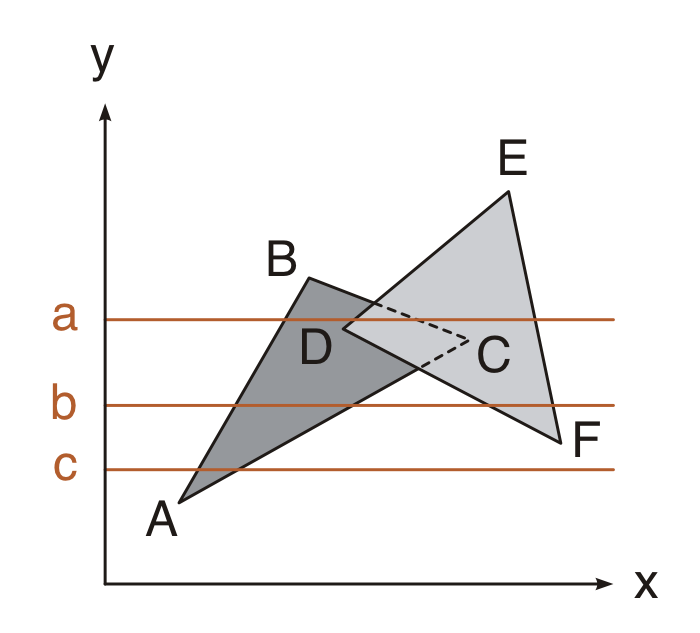
\includegraphics[width=0.7\columnwidth]{Figures/09.png}
    \caption{Algoritmo Scanline}
    \label{fig:figure}
\end{figure}
Tutti i poligoni da renderizzare sono ordinate dall'alto sulla asse delle ordinate in ordine di apparizione. Poi, per ogni riga o scanline dell'immagine è calcolato utilizzando l'intersezione di una scanline con i poligoni nella parte anteriore della lista ordinata, mentre quest'ultima viene aggiornata scartando i poligoni non più visibile man mano che la scanline attiva avanza verso il basso dell'immagine.\\
Il vantaggio principale di questo metodo è che l'ordine dei vertici lungo la normale del piano di scansione riduce il numero di comparazioni tra i bordi. Un ulteriore vantaggio rispetto allo z-buffering è che il processo dei pixel visibili è mantenuto al minimo assoluto. Attraverso l'ordinamento front-to-back utilizzato nei moderni sistemi z-buffer, si possono realizzare benefici simile. 

\subsection{Z-buffering}
Lo Z-buffering, anche noto come depth buffering, è la gestione delle coordinate di profondità delle immagini nella 3D graphics, fatta di solito a livello hardware. Quando si proietta un oggetto sullo schermo con un motore di 3D-rendering, la profondità (z-value) del pixel generato nell'immagine proiettata viene memorizzata in un buffer (z-buffer). Un z-value corrisponde alla misura della distanza perpendicolare da un pixel sul piano di proiezione alla sua corrispondete coordinata 3D su un poligono nello spazio. Lo Z-buffer ha la stessa struttura di un immagine, ovvero un 2D-array, con la sola differenza che memorizza uno z-value per ogni pixel dello schermo invece che dei pixel dei dati. Ha la stesse dimensioni di uno screen buffer, eccetto quando sono utilizzati Z-buffer multipli. \\
Quando vediamo un immagine contenente oggetti o superfici parzialmente o totalmente opachi, non è possibile vedere completamente questi oggetti sia che siano lontani dall'osservatore sia che siano dietro altri oggetti. L'identificazione e la rimozioni di tali oggetti è chiamato problema delle superfici nascoste (hidden surface problem). Per migliorare il tempo di rendering, le superfici nascoste vengono rimosse prima che l'immagina sia memorizzata nel z-buffer, in modo che quest'ultimo calcoli lo z-value del pixel corrispondente al primo oggetto che compare e lo compara con lo z-value del pixel nella stessa posizione nel z-buffer corrispondente all'oggetto che è più vicino all'osservatore per trovare la sovrapposizione.
\subsection{Algoritmo del pittore}
L'algoritmo del pittore è una delle soluzioni più semplici al problema della visibilità nella 3D computer graphics. Quando proietti una scena 3D in un piano 2D, è necessario decidere quale  tra i poligoni è visibile. 
\begin{figure}[H]
    \centering
    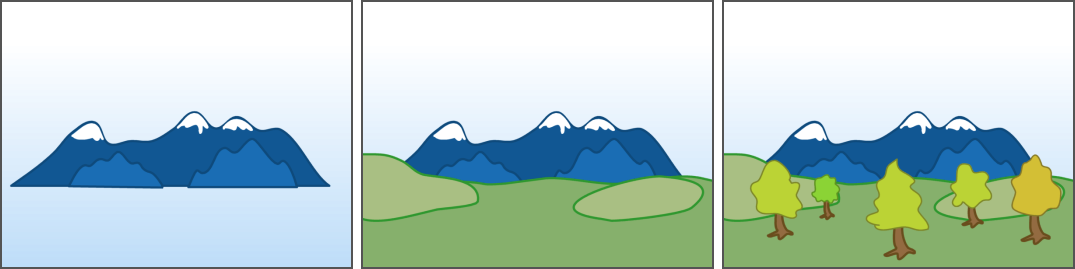
\includegraphics[width=0.7\columnwidth]{Figures/10.png}
    \caption{Algoritmo del pittore}
    \label{fig:figure}
\end{figure}
L'algoritmo del pittore ordina tutti i poligoni nella scena partendo dalla profondità e poi li disegna in questo ordine, dal più lontano al più vicino. Si disegna sulle parti non visibili, al costo di avere oggetti già disegnati al nascosti. L'ordine usato dall'algoritmo è chiamato depth order: se un oggetto oscura la parte di un altro, allora il primo oggetto disegnato dopo il secondo viene oscurato. 

\section{Ray Tracing}
Negli ultimi anni, la qualità delle immagini generate computazionalmente hanno raggiunto un livello di realismo tale che i rendering sono indistinti dalle fotografie.\\
Nella computer graphics, il ray tracing è una tecnica di rendering per generare un'immagine tracciando il percorso della luce come pixel in un piano e simulando gli effetti dati dall'intersezione di tale percorso con gli oggetti virtuali. La tecnica può produrre un grado di realismo visivo molto alto, anche più alto a volte dei tipici metodi di rendering scanline ma con un alto costo computazionale. \\
Avanzati effetti di shading possono rendere la visualizzazione più efficace. Il vantaggio, l'opportunità e l'obiettivo del ray tracing è quello di fornire ulteriori segnali visivi per una migliore visualizzazione degli oggetti 3D.\\
Ci sono almeno quattro diversi raggi coinvolti nel ray tracing:
\begin{itemize}
	\item \textbf{Raggi oculari} che hanno origine dagli occhi.
	\item \textbf{Raggi d'ombra}: dal punto di superficie alla sorgente di luce.
	\item \textbf{Raggi di riflessione}: dal punto di superficie in direzione dello specchio.
	\item \textbf{Raggi di trasmissione}: dal punto di superficie nella direzione di rifrazione.
\end{itemize}
L'algoritmo di ray tracing calcola il raggio dell'occhio dell'osservatore attraverso ogni pixel, calcola il punto di intersezione più vicina con una superficie di scena, quindi ombreggia quel punto calcolando i raggi d'ombra e genera i raggi riflessi e rifratti.
\begin{figure}[H]
    \centering
    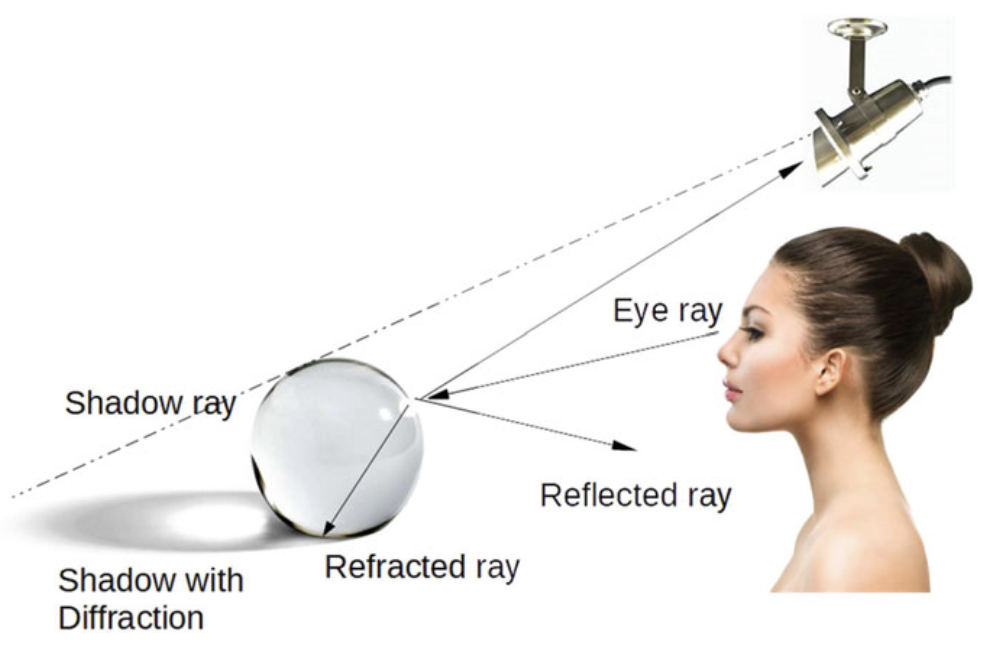
\includegraphics[width=0.7\columnwidth]{Figures/11.png}
    \caption{Raggi nel ray tracing}
    \label{fig:figure}
\end{figure}
Il ray tracing ricorsivo simula la riflessione speculare e le ombre attraverso e fuori dalle superfici trasparenti. Può usare o impiegare l'illuminazione indiretta, a volte aree di sorgenti luminosa o altre influenze caustiche.\\
Crea riflessi accurati, rifrazioni, ombre e altre caratteristiche che possano far sembrare la scena reale.\\
Il ray tracing in grandi linee può essere diviso in tre generali categorie:
\begin{enumerate}
	\item Off-line
	\item Interactive
	\item Real-time
\end{enumerate}
Off-line è usato ampiamente dagli studi cinematografici, pubblicitari e di design. Ha la qualità maggiore.\\
Interactive ray tracing riduce il numeri di raggi in modo da avere comunque una buona immagine e allo stesso tempo di offrire all'utente la possibilità di manipolare il modello.\\
Real-time ray tracing può essere realizzato, con alcune restrizioni, dall'assistenza di piccoli supercomputer.
\begin{figure}[H]
    \centering
    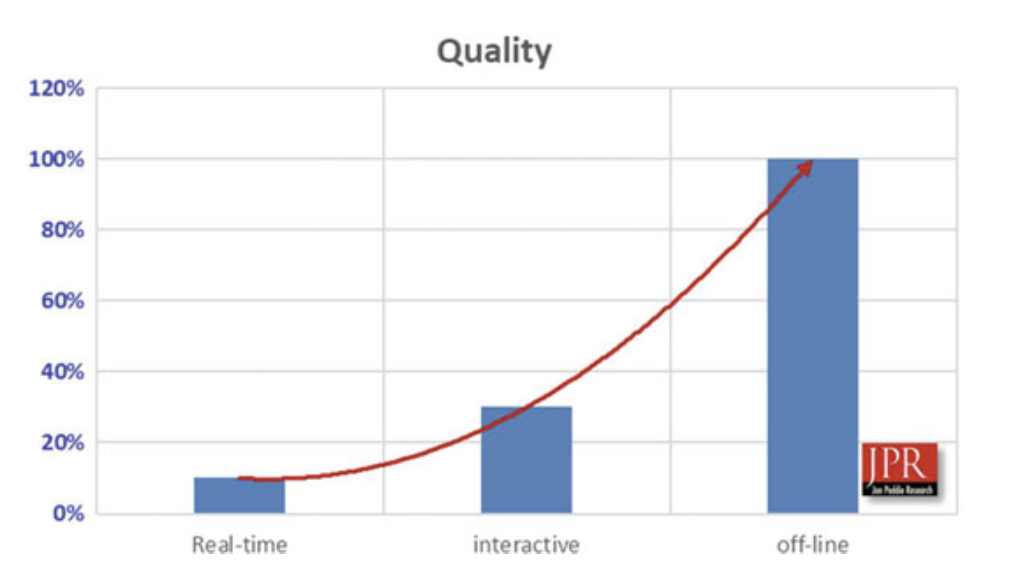
\includegraphics[width=0.7\columnwidth]{Figures/12.png}
    \caption{Performance e qualità nei vari modi di ray tracing}
    \label{fig:figure}
\end{figure}
Uno dei trucchi del ray tracing è quello di tracciare solo determinati elementi o oggetti all'interno di un'immagine ma, se fatto in modo giusto, si ha un immagine fisicamente corretta.  
\begin{figure}[H]
    \centering
    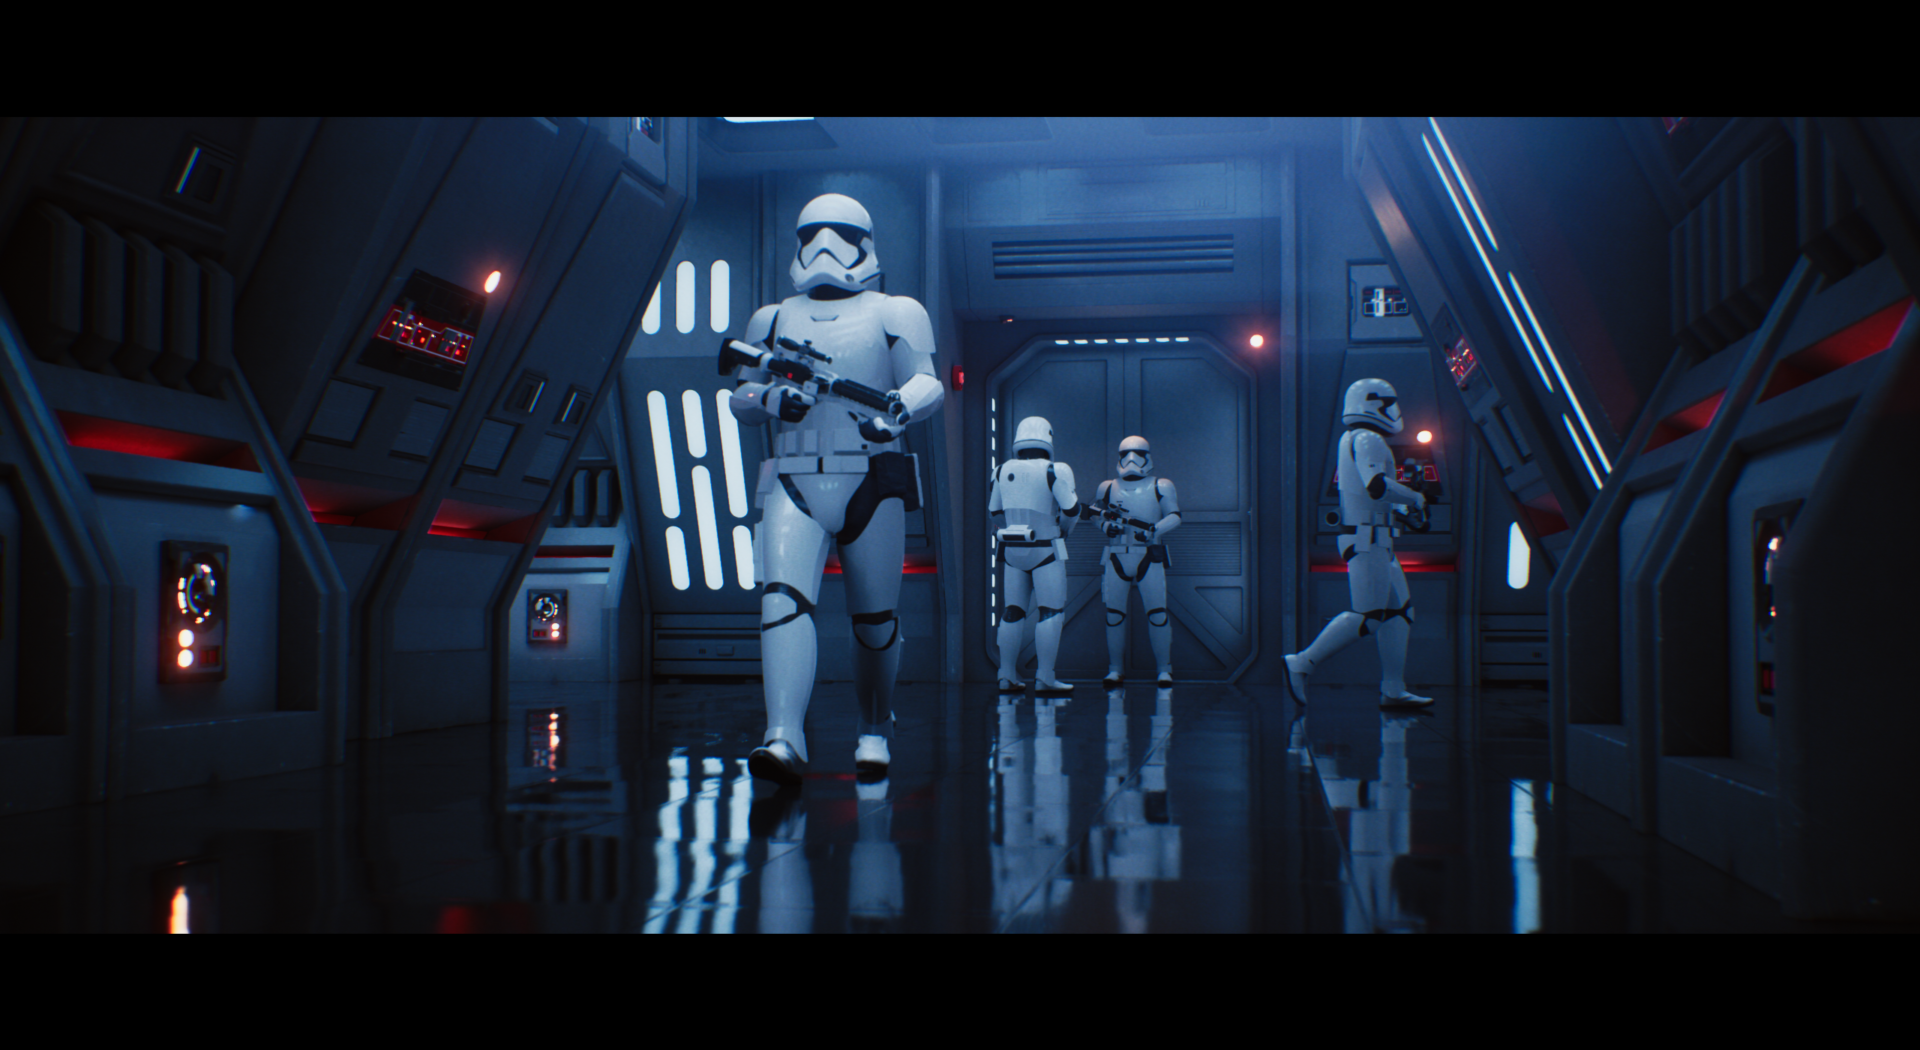
\includegraphics[width=0.7\columnwidth]{Figures/13.png}
    \caption{Stormtroopers (Star Wars) renderizzati con real-time ray tracing (Nvidia): il background non ha applicato il ray tracing, ne tanto meno lo necessita, ma il pavimento potrebbe dipendere dal materiale che il l'autore decida di utilizzare}
    \label{fig:figure}
\end{figure}
Il ray tracing è capace di simulare una vasta varietà di effetti ottici, ad esempio riflessione, rifrazione e fenomeni di dispersione, ma non è necessariamente il metodo più realistico: metodi che includono tecniche addizionali posso dare simulazioni più accurate. \\
Il ray tracing è imperfetto: immagini con un ray tracing basico sono molto pulite, quindi l'allineamento degli oggetti e il campionamento possono portare a pattern non intenzionali noti come pattern di moiré e aliasing. \\
Il ray tracing dà colore per ogni possibile punto dell'immagine. Tuttavia un pixel quadrato contiene un numero infinito di punti e quei punti potrebbero non avere tutti lo stesso colore. Il campionamento viene utilizzato appunto per scegliere il colore di tale pixel, ma come è ben noto, il campionamento implica aliasing.

\section{Path Tracing}
\taustart{I}l Path Tracing è un'estensione dell'algoritmo del ray tracing. Esso simula molti percorsi di luce per ogni pixel e ne valuta la media per calcolare il colore finale per ognuno di essi.\\
Ogni volta che un raggio colpisce una superficie, un nuovo raggio viene tracciato a partire dal punto di collisione in direzione casuale fino a quando raggiunge una massima profondità di percorso (maximum path depth) o finche un meccanismo "uccide" il raggio (simile ad una roulette russa). Di conseguenza, il Path Tracing produce effetti come mescolamento dei colori diffuso (diffuse color bleedind), riflessi lucisi (sfocati), ombre morbide, reali luci di area, vera profondità di campo.\\
Path Tracing usa il campionamento casuale (metodo Monte Carlo) per incrementare il calcolo dell'immagine finale: il processo di campionamento casuale consente di rendere alcuni fenomeni complessi che non vengono gestiti nel ray tracing regolare, ma generalmente ci vuole più tempo per produrre un'immagine tracciata di alta qualità. \\
Tale campionamento introduce del rumore nell'immagine renderizzata. Tale problema si risolve lasciando che l'algoritmo generi più campioni.

\subsection{Differenze tra Path Tracing e Ray Tracing}
Path Tracing si basa fisicamente sulla simulazione della luce che consente un rendering altamente realistico. \'E un algoritmo elegante che può simulare molti complessi modi di determinare il percorso e la dispersione della luce nelle scene virtuali. Il Path Tracing usa il tracciamento dei raggi per determinare la visibilità tra gli eventi di scattering. Ray Tracing è una operazione di base che può essere usata per molteplici cose. Quindi, il tracciamento dei raggi da solo non produce in maniera automatica immagini realistiche. Per questo si utilizzano algoritmi del trasporto della luce come il Path Tracing. Tuttavia, anche se elegante e molto potente, il Path Tracing è molto costoso e impiega parecchio tempo per produrre immagini stabili. A tal caso sono stati proposti dei filtri adattivi che riutilizzano più informazioni possibili su molti fotogrammi e pixel al fine di produrre immagini robuste e stabili.

\subsection{Rumore nel Ray Tracing}
I rendering in real-time tramite GPU utilizzano la rasterizzazione o ciò che è noto come rendering scanline. Per fornire un rendering in tempo reale, i motori di gioco e altri render usano tecniche intelligenti, ma sono falsi o approssimazioni: chiunque usi tali strumenti sa immediatamente quali sono queste limitazioni e il lavoro extra necessario per cercare di approssimare gli effetti desiderati. Il rendering real-time non può creare reali riflessi, rifrazioni, o rimbalzi di luce. Per generare tali effetti di luce, vi è la necessità di approssimare o imitare tali effetti.\\
Invece di tracciare da centinaia a migliaia di raggi per pixel, per minimizzare i tempi, è stata sviluppata una tecnica chiamata denoising: il concetto è quello di seguire pochi raggi per diminuire il rumore dell'immagine. Ci sono due metodi di denoising:
\begin{itemize}
	\item \textbf{Temporal denoising} renderizza alcuni raggi per ogni frame; essi sono diversi, e nel tempo, la loro media da un risultato fluido. Per un immagine ferma, il temporal denoising funziona bene, ma per un'immagine in movimento ci sono problemi con il ghosting. 
	\item \textbf{Spatial denoising} viene applicato alle aree rumorose e utilizza un filtro di levigatura su di esse come una sfocatura del bordo. Non funziona bene con l'animazione e crea macchie in movimento. Rimuove anche la nitidezza dagli oggetti che dovrebbero essere nitidi, pertanto viene utilizzato il denoising spaziale. Il denoising spaziale combina i risultati di più pixel vicini come un filtro di sfocatura. Tuttavia, crea luccichii sulle immagini in movimento.
\end{itemize}

\section{Applicazione}
\taustart{D}i seguito viene presentata una semplice implementazione del ray tracing in Python. 

\subsection{Prerequisiti}
Quello che necessità sono basiche nozioni di geometria vettoriale:
\begin{itemize}
	\item Dati due punti $A$ e $B$, qualunque sia la dimensione $(1, 2, 3, \dots, n)$, il vettore che va da $A$ a $B$ può essere calcolato con $B-A$.
	\item La lunghezza del vettore (norma), che si valuta calcolando la radice quadrata della somma delle componenti vettoriali al quadrato. Si denota con $\Vert v \Vert$.
	\item Versore, vettore di lunghezza 1: $\Vert v \Vert=1$. Il versore di un vettore può essere calcolato effettuando una normalizzazione: $u=\frac{v}{\Vert v \Vert}$.
	\item Prodotto tra vettori.
	\item Risoluzione di equazioni di secondo grado
\end{itemize}

\section{Algoritmo}
Per dare una spiegazione dell'algoritmo vi è la necessità di impostare la scena:
\begin{itemize}
	\item Impostiamo oggetti nello spazio 3D
	\item Impostiamo una sorgente di luce
	\item Vi è la necessità di impostare un punto (o camera) per osservare la scena
	\item Affinché la camera osservi, è necessario uno schermo, attraverso il quale osservare gli oggetti
\end{itemize} 

\begin{figure}[H]
    \centering
    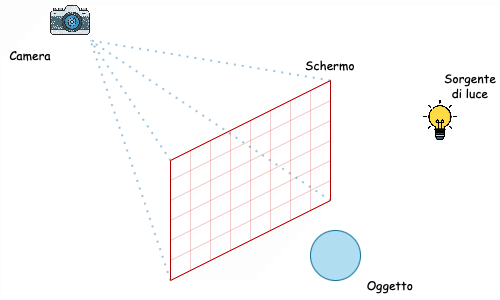
\includegraphics[width=0.7\columnwidth]{Figures/14.png}
    \caption{}
    \label{fig:figure}
\end{figure}

Dato la scena, l'algoritmo del ray tracing 
\begin{algorithm}
  \caption{Algoritmo del ray tracing}\label{r_t}
  \begin{algorithmic}
  	\ForAll{pixel $p(x,y,z)$ dello schermo}
        \State $p \leftarrow$ il colore nero 
        \If{il raggio che parte dalla camera e  p interseca un oggetto della scena}
         	\State Calcola il punto d'intersezione con l'oggetto più vicino
         	\If{non ci sono oggetti tra il punto d'intersezione e la luce} 
         		\State calcola il colore del punto d'intersezione
         		\State $ p \leftarrow$  colore del punto d'intersezione
         	\EndIf	
        \EndIf
    \EndFor
  \end{algorithmic}
\end{algorithm}

\begin{figure}[H]
    \centering
    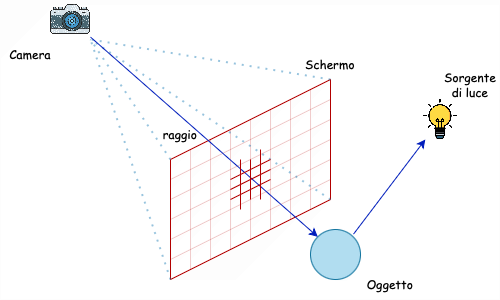
\includegraphics[width=0.7\columnwidth]{Figures/15.png}
    \caption{}
    \label{fig:figure}
\end{figure}

Alla fine dell'algoritmo lo schermo si riempierà con il corretto colore e l'immagina può essere salvata.

\subsection{Configurazione della scena}
Prima di tutto è necessario configurare la scena.
Supponiamo che camera e schermo siano posizionati come in figura.
\begin{figure}[H]
    \centering
    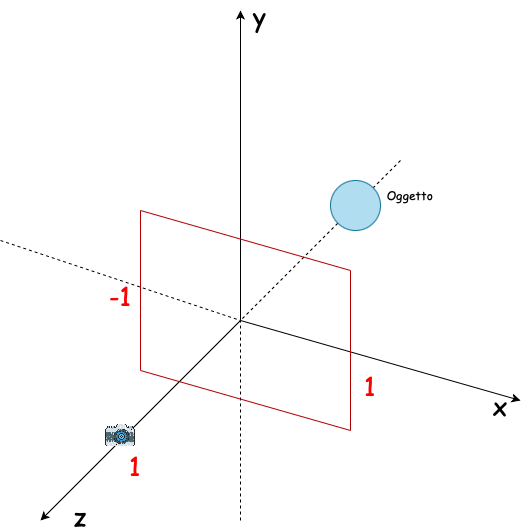
\includegraphics[width=0.7\columnwidth]{Figures/16.png}
    \caption{Scena}
    \label{fig:figure}
\end{figure}
Da qui, la camera si trova in $\left(x=0, y=0, z=1\right)$ e lo schermo è parte del piano formato dall'asse $x$ e $y$.\\
Può essere qui scritto uno scheletro del codice.

\begin{lstlisting}[language=Python]
import numpy as np
import matplotlib.pyplot as plt

width = 500
height = 300

camera = np.array([0, 0, 1])
ratio = float(width) / height
screen = (-1, 1/ratio, 1, -1/ratio)

image = np.zeros((height, width, 3))
for i, y in enumerate(np.linspace(screen[1], screen[3], height)):
    for j, x in enumerate(np.linspace(screen[0], screen[2], width)):
        # image[i, j] = ...
    print("progress: %d/%d" % (i+1, height))

plt.imsave('image.png', image)
\end{lstlisting}

\begin{itemize}
	\item La camera è solo una posizione (3 coordinate)
	\item Lo schermo è definito da quattro numeri: sinistra, sopra, destra, sotto. \'E compreso tra $-1$ e $1$ sull'asse delle $x$ (valore arbitrario), ed è compreso  da $\frac{-1}{ratio}$ e $\frac{1}{ratio}$ sull'asse delle $y$, dove il $ratio = \frac{image\_width}{image\_height}$. Si fa ciò poiché si vuole l' aspect ratio del nostro schermo corrisponda con quella dell'immagine che si vuole produrre.
	\item Il loop divide lo schermo lungo altezze e larghezza in punti, appartenenti al piano $x-y$, per poi calcolare il colore di ogni singolo pixel.
\end{itemize}

Facendo eseguire tale scheletro l'immagine di output è completamente nera.

\subsection{Intersezione dei raggi}
Visto che il raggio inizia dalla fotocamera e va nella direzione del pixel mirato in quel momento, possiamo definire un versore che punta in una direzione simile. Pertanto, si definisce un raggio che partendo dalla camera e va verso il pixel con la seguente equazione:
\begin{equation*}
	ray(t) = camera + \frac{pixel - camera}{\Vert pixel - camera \Vert} t
\end{equation*}
Si ricordi, la fotocamera e il pixel sono punti nello spazio tridimensionale. Per $t=0$ si ha la posizione della camera, mentre all'aumentare di $t$ più ci si allontana dalla camera nella direzione del pixel.\\
Possiamo generalizzare l'equazione precedente indicando con $O$ l'origine e $D$ la destinazione:
\begin{equation*}
	ray(t) = O + \frac{D - O}{\Vert D -O \Vert} t = O + d\cdot t
\end{equation*} 
con $d$ il vettore di direzione.\\

Possiamo quindi aggiungere al codice precedente il codice relativo al calcolo del raggio.
\begin{lstlisting}[language=Python]
import numpy as np
import matplotlib.pyplot as plt

def normalization(vector):
    return vector / np.linalg.norm(vector)

width = 500
height = 300

camera = np.array([0, 0, 1])
ratio = float(width) / height
screen = (-1, 1/ratio, 1, -1/ratio)     

image = np.zeros((height, width, 3))
for i, y in enumerate(np.linspace(screen[1], screen[3], height)):
    for j, x in enumerate(np.linspace(screen[0], screen[2], width)):
        pixel = np.array([x, y, 0])
        origin = camera
        direction = normalization(pixel - origin)

        # image[i, j] = ...
        
    print("progress: %d/%d" % (i+1, height))
    
plt.imsave('image.png', image)
\end{lstlisting}

\begin{itemize}
	\item \'E stata aggiunta una funzione chiamata \texttt{normalization(vector)} per normalizzare il vettore
	\item \'E stato aggiunto il calcolo dell'origine e della direzione;il pixel ha $z=0$ poiché si trova sullo schermo che si trova su piano $x-y$.
\end{itemize}

\subsection{Definizione della sfera}
La parte più complessa l'intersezione con gli oggetti di scena, poiché essa differisce in base alla tipologia di oggetto. Per semplicità, in tale esempio si prende in considerazione una sfera.\\
Una sfera è un oggetto molto semplice da definire matematicamente: essa è definita come un insieme di punti che sono tutti alla stessa distanza $r$ (raggio) da un dato punto (centro). Quindi, da un centro $C$ di una sfera, e il suo raggio $r$, un arbitrario punto $X$ si trova sulla sfera se e solo se:
\begin{equation*}
	\Vert X - C \Vert^2 = r^2
\end{equation*}
Possiamo quindi già definire nel codice la nostra sfera come segue (la inseriamo dopo la dichiarazione dello schermo)

\begin{lstlisting}[language=Python]
objects = [
    {'center': np.array([-0.2, 0, -1]), 'radius':0.7},
    {'center': np.array([0.1, -0.3, 0]), 'radius':0.1},
    {'center': np.array([-0.3, 0, 0]), 'radius':0.15}
]
\end{lstlisting}

\subsection{L'intersezione con la sfera}
Conoscendo l'equazione dei raggi e sapendo la condizione che va soddisfatta affinché un punto si trovi sulla superficie sferica, sostituendo la prima di queste nella seconda, si ha:
\begin{equation*}
	\begin{split}
		&\Vert ray(t) - C\Vert^2 = r^2\\
		\implies & \Vert O + d\cdot t - C \Vert^2 = r^2 \\
		\implies & \langle d\cdot t + O - C, d\cdot t + O - C\rangle = r^2 \\
		\implies & \langle d, d\rangle t^2 + 2t\langle d, O-C\rangle + \langle O-C, O-C\rangle = r^2 \\
		\implies & \Vert d\Vert ^2 t^2 + 2t\langle d, O-C \rangle + \Vert O-C\Vert ^2 - r^2 = 0
	\end{split}
\end{equation*}

Questa è un'equazione di secondo grado che può essere risolta per $t$. Il discriminante è:
\begin{equation*}
	\begin{split}
		& a = \Vert d \Vert ^2 = 1\\
		& b = 2 \langle d, O-C \rangle\\
		& c = \Vert O-C \Vert ^2 - r^2 \\
		& \Delta = b^2 - 4ac
	\end{split}
\end{equation*}

Una volta calcolato il discriminante, ci sono tre possibilità:

\begin{figure}[H]
    \centering
    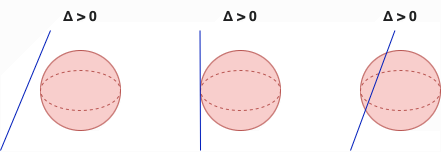
\includegraphics[width=0.7\columnwidth]{Figures/17.png}
    \caption{}
    \label{fig:figure}
\end{figure}
Viene utilizzato il terzo caso ($\Delta > 0$), ovvero l'unico caso in cui si verificano intersezioni. La funzione, che ritorna il valore \texttt{t}, distanza tra l'origine del raggio e il punto d'intersezione, se si verifica $\Delta<0$, o valore \texttt{None} in caso contrario, è così definita:
\begin{lstlisting}[language=Python]
def sphere_intersect(center, radius, ray_origin, ray_direction):
    b = 2* np.dot(ray_direction, ray_origin - center)
    c = np.linalg.norm(ray_origin - center) ** 2 - radius ** 2
    delta = b**2 - 4*c
    if delta > 0:
        t1 = (-b + np.sqrt(delta)) / 2
        t2 = (-b - np.sqrt(delta)) / 2
        if t1 > 0 and t2 > 0:
            return min(t1, t2)
    return None
\end{lstlisting}
Va notato che si ritorna solo la soluzione più piccola tra le due, che indica l'intersezione più vicina, se ovviamente entrambe le soluzioni sono positive.

\subsection{Intersezione con l'oggetto più vicino}
Può essere creata facilmente, utilizzando la funzione precedente, un funzione che cerca l'oggetto più vicino che viene intercettato dal raggio, se esiste. Semplicemente, si valutano tutte le sfere in cerca di intersezioni, memorizzando la più vicina.
\begin{lstlisting}
def nearest_intersected_object(objects, ray_origin, ray_direction):
    distances = [sphere_intersect(obj['center'], obj['radius'], ray_origin, ray_direction) for obj in objects]
    nearest_object = None
    min_distance = np.inf
    for index, distance in enumerate(distances):
        if distance and distance < min_distance:
            min_distance = distance
            nearest_object = objects[index]
    return nearest_object, min_distance
\end{lstlisting}
Alla chiamata di tale funzione, se l'oggetto più vicino non esiste, non c'è nessun oggetto che viene intersecato dal raggio, mentre in caso contrario viene ritornato l'oggetto più vicino con la rispettiva distanza.

\subsection{Punti d'intersezione}
Utilizzando le funzioni mostrate finora, si possono calcolare i punti d'intersezione.
\begin{lstlisting}[language=Python]
import numpy as np
import matplotlib.pyplot as plt

def normalization(vector):
    return vector / np.linalg.norm(vector)

def sphere_intersect(center, radius, ray_origin, ray_direction):
    b = 2* np.dot(ray_direction, ray_origin - center)
    c = np.linalg.norm(ray_origin - center) ** 2 - radius ** 2
    delta = b**2 - 4*c
    if delta > 0:
        t1 = (-b + np.sqrt(delta)) / 2
        t2 = (-b - np.sqrt(delta)) / 2
        if t1 > 0 and t2 > 0:
            return min(t1, t2)
    return None

def nearest_intersected_object(objects, ray_origin, ray_direction):
    distances = [sphere_intersect(obj['center'], obj['radius'], ray_origin, ray_direction) for obj in objects]
    nearest_object = None
    min_distance = np.inf
    for index, distance in enumerate(distances):
        if distance and distance < min_distance:
            min_distance = distance
            nearest_object = objects[index]
    return nearest_object, min_distance

width = 500
height = 300

camera = np.array([0, 0, 1])
ratio = float(width) / height
# sinistra, sopra, destra, sotto
screen = (-1, 1/ratio, 1, -1/ratio)  

objects = [
    {'center': np.array([-0.2, 0, -1]), 'radius':0.7},
    {'center': np.array([0.1, -0.3, 0]), 'radius':0.1},
    {'center': np.array([-0.3, 0, 0]), 'radius':0.15}
]

image = np.zeros((height, width, 3))
for i, y in enumerate(np.linspace(screen[1], screen[3], height)):
    for j, x in enumerate(np.linspace(screen[0], screen[2], width)):
        pixel = np.array([x, y, 0])
        origin = camera
        direction = normalization(pixel - origin)

        # check for intersections
        nearest_object, min_distance = nearest_intersected_object(objects, origin, direction)
        if nearest_object is None:
            continue

        # compute intersection point between ray and nearest object
        intersection = origin + min_distance*direction
        
    # image[i, j] = ...  
    print("progress: %d/%d" % (i+1, height))

plt.imsave('image.png', image)
\end{lstlisting}

\subsection{Intersezione della luce}
Finora si è visto che se c'è una linea che parte dalla camera verso un oggetto, si sa qual è e che parte di esso si sta osservando. Non si sa se quell'oggetto sia illuminato o meno. Potrebbe capitare che la luce non colpisca quello specifico punto e quindi non può essere visto. Va quindi controllato se non c'è alcun oggetto della scena tra il punto d'intersezione e la luce.\\
Si vuole sapere se il raggio che parte dal punto d'intersezione e va verso la luce interseca un oggetto della scena prima di attraversare la luce (utilizziamo la funzione\texttt{nearest\_intersected\_object()}). 

Si dichiari la luce come segue:
\begin{lstlisting}[language=Python]
light = {'position': np.array([5, 5, 5])}
\end{lstlisting}
Per verificare se un oggetto sta ombreggiando il punto d'intersezione, va fatto passare il raggio che inizia dal punto d'intersezione e va verso la luce, e vedere se l'oggetto più vicino restituito è effettivamente più vicino della luce al punto d'intersezione, in altre parole nel mezzo.
\begin{lstlisting}
# ...
intersection = origin + min_distance*direction

 intersection_to_light = normalization(light['position'] - intersection)

_, min_distance = nearest_intersected_object(objects, intersection, intersection_to_light)
intersection_to_light_distance = np.linalg.norm(light['position'] - intersection)
is_shadowed = min_distance < intersection_to_light_distance
\end{lstlisting}

Questo non funzionerà perché c'è bisogno di una piccola modifica: se si usasse il punto di intersezione come origine, potrebbe essere rilevata la sfera come oggetto tra il punto d'intersezione e la luce. Una soluzione è quella di allontanarsi leggermente dalla sfera nella direzione del vettore normale della superficie.
\begin{figure}[H]
    \centering
    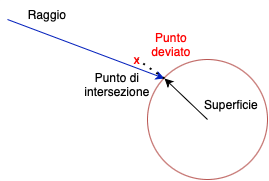
\includegraphics[width=0.7\columnwidth]{Figures/18.png}
    \caption{}
    \label{fig:figure}
\end{figure}
Questa procedura può essere utilizzata per ogni tipo di oggetto.\\
Il codice corretto sarà quindi:
\begin{lstlisting}[language=Python]
# ...
intersection = origin + min_distance*direction

normal_to_surface = normalization(intersection - nearest_object['center'])
shifted_point = intersection + 1e-6*normal_to_surface
intersection_to_light = normalization(light['position'] - shifted_point)

_, min_distance = nearest_intersected_object(objects, shifted_point, intersection_to_light)
intersection_to_light_distance = np.linalg.norm(light['position'] - intersection)
is_shadowed = min_distance < intersection_to_light_distance
        
if is_showed:
	continue
\end{lstlisting}

\subsection{Modello di riflessione: Blinn-Phong}
Finora si è visto che un fascio di luce colpisce un oggetto e il riflesso viene intravisto va verso la camera. Ma cosa vede la camera? Per rispondere a tale domanda interviene il modello di Blinn-Phong.\\
Il modello di Blinn-Phong è un'approssimazione del modello Phong che è computazionalmente più leggero.\\
In accordo con tale modello, ogni materiale ha 4 proprietà:
\begin{itemize}
	\item \textbf{Colore ambientale}: colore dell'oggetto in assenza di luce;
	\item \textbf{Colore diffuso}: colore percepito come risultato della riflessione diffusa della luce;
	\item \textbf{Colore speculare}: colore di una parte lucida di un oggetto quando è colpito dalla luce;
	\item \textbf{Lucentezza}: coefficiente che indica quanto lucida è una superficie.
\end{itemize}
Quindi ogni oggetto deve avere queste proprietà, che aggiungiamo al codice

\begin{lstlisting}[language=Python]
objects = [
    {'center': np.array([-0.2, 0, -1]), 'radius':0.7, 'ambient': np.array([0.1, 0, 0]), 'diffuse': np.array([0.7, 0, 0]), 'specular': np.array([1, 1, 1]), 'shininess':100},
    {'center': np.array([0.1, -0.3, 0]), 'radius':0.1, 'ambient': np.array([0.1, 0, 0.1]), 'diffuse': np.array([0.7, 0, 0.7]), 'specular': np.array([1, 1, 1]), 'shininess':100},
    {'center': np.array([-0.3, 0, 0]), 'radius':0.15, 'ambient': np.array([0, 0.1, 0]), 'diffuse': np.array([0, 0.6, 0]), 'specular': np.array([1, 1, 1]), 'shininess':100}
]
\end{lstlisting}

Tale modello impone queste proprietà anche alla luce, eccetto per la lucentezza.
\begin{lstlisting}[language=Python]
light = {'position': np.array([5, 5, 5]), 'ambient': np.array([1, 1, 1]), 'diffuse': np.array([1, 1, 1]), 'specular':np.array[1, 1, 1]}
\end{lstlisting}
Date queste proprietà, il modello Blinn-Phong calcola l'illuminazione di un singolo pixel come segue:
\begin{equation*}
	I_p = k_a \cdot i_a + k_d \cdot i_d \cdot L \cdot N + k_s \cdot i_s \cdot \left( N \cdot \frac{L+V}{\Vert L + V \Vert} \right)^{\frac{\alpha}{4}}
\end{equation*}
dove
\begin{enumerate}
	\item $k_a$, $k_d$, $k_s$ sono le proprietà ambientali, di diffusione, speculari di un oggetto;
	\item $i_a$, $i_d$, $i_s$ sono le proprietà ambientali, di diffusione, speculari della luce;
	\item $L$ è la direzione del versore che parte dal punto d'intersezione verso la luce;
	\item $N$ è il versore della normale della superficie nel punto d'intersezione;
	\item $V$ il versore che va dal punto d'intersezione verso la camera
	\item $\alpha$ è la lucentezza dell'oggetto
\end{enumerate}

\begin{lstlisting}[language=Python]
if is_shadowed:
            break

# RGB
illumination = np.zeros((3))

# ambient
illumination += nearest_object['ambient'] * light['ambient']

# diffuse
illumination += nearest_object['diffuse'] * light['diffuse'] * np.dot(intersection_to_light, normal_to_surface)

# specular
intersection_to_camera = normalization(camera - intersection)
H = normalization(intersection_to_light + intersection_to_camera)
illumination += nearest_object['specular'] * light['specular'] * np.dot(normal_to_surface, H) ** (nearest_object['shininess']/4)

image[i, j] = np.clip(illumination, 0, 1) 
\end{lstlisting}
Nel l'ultima linea di codice è stato limitato il colore tra 0 e 1 per non avere problemi.\\
\subsection{Primo risultato}
Eseguendo il codice, incrementando altezza e larghezza dello schermo (comporta un aumento del tempo di calcolo), quello che si ottiene è la seguente immagine
\begin{figure}[H]
    \centering
    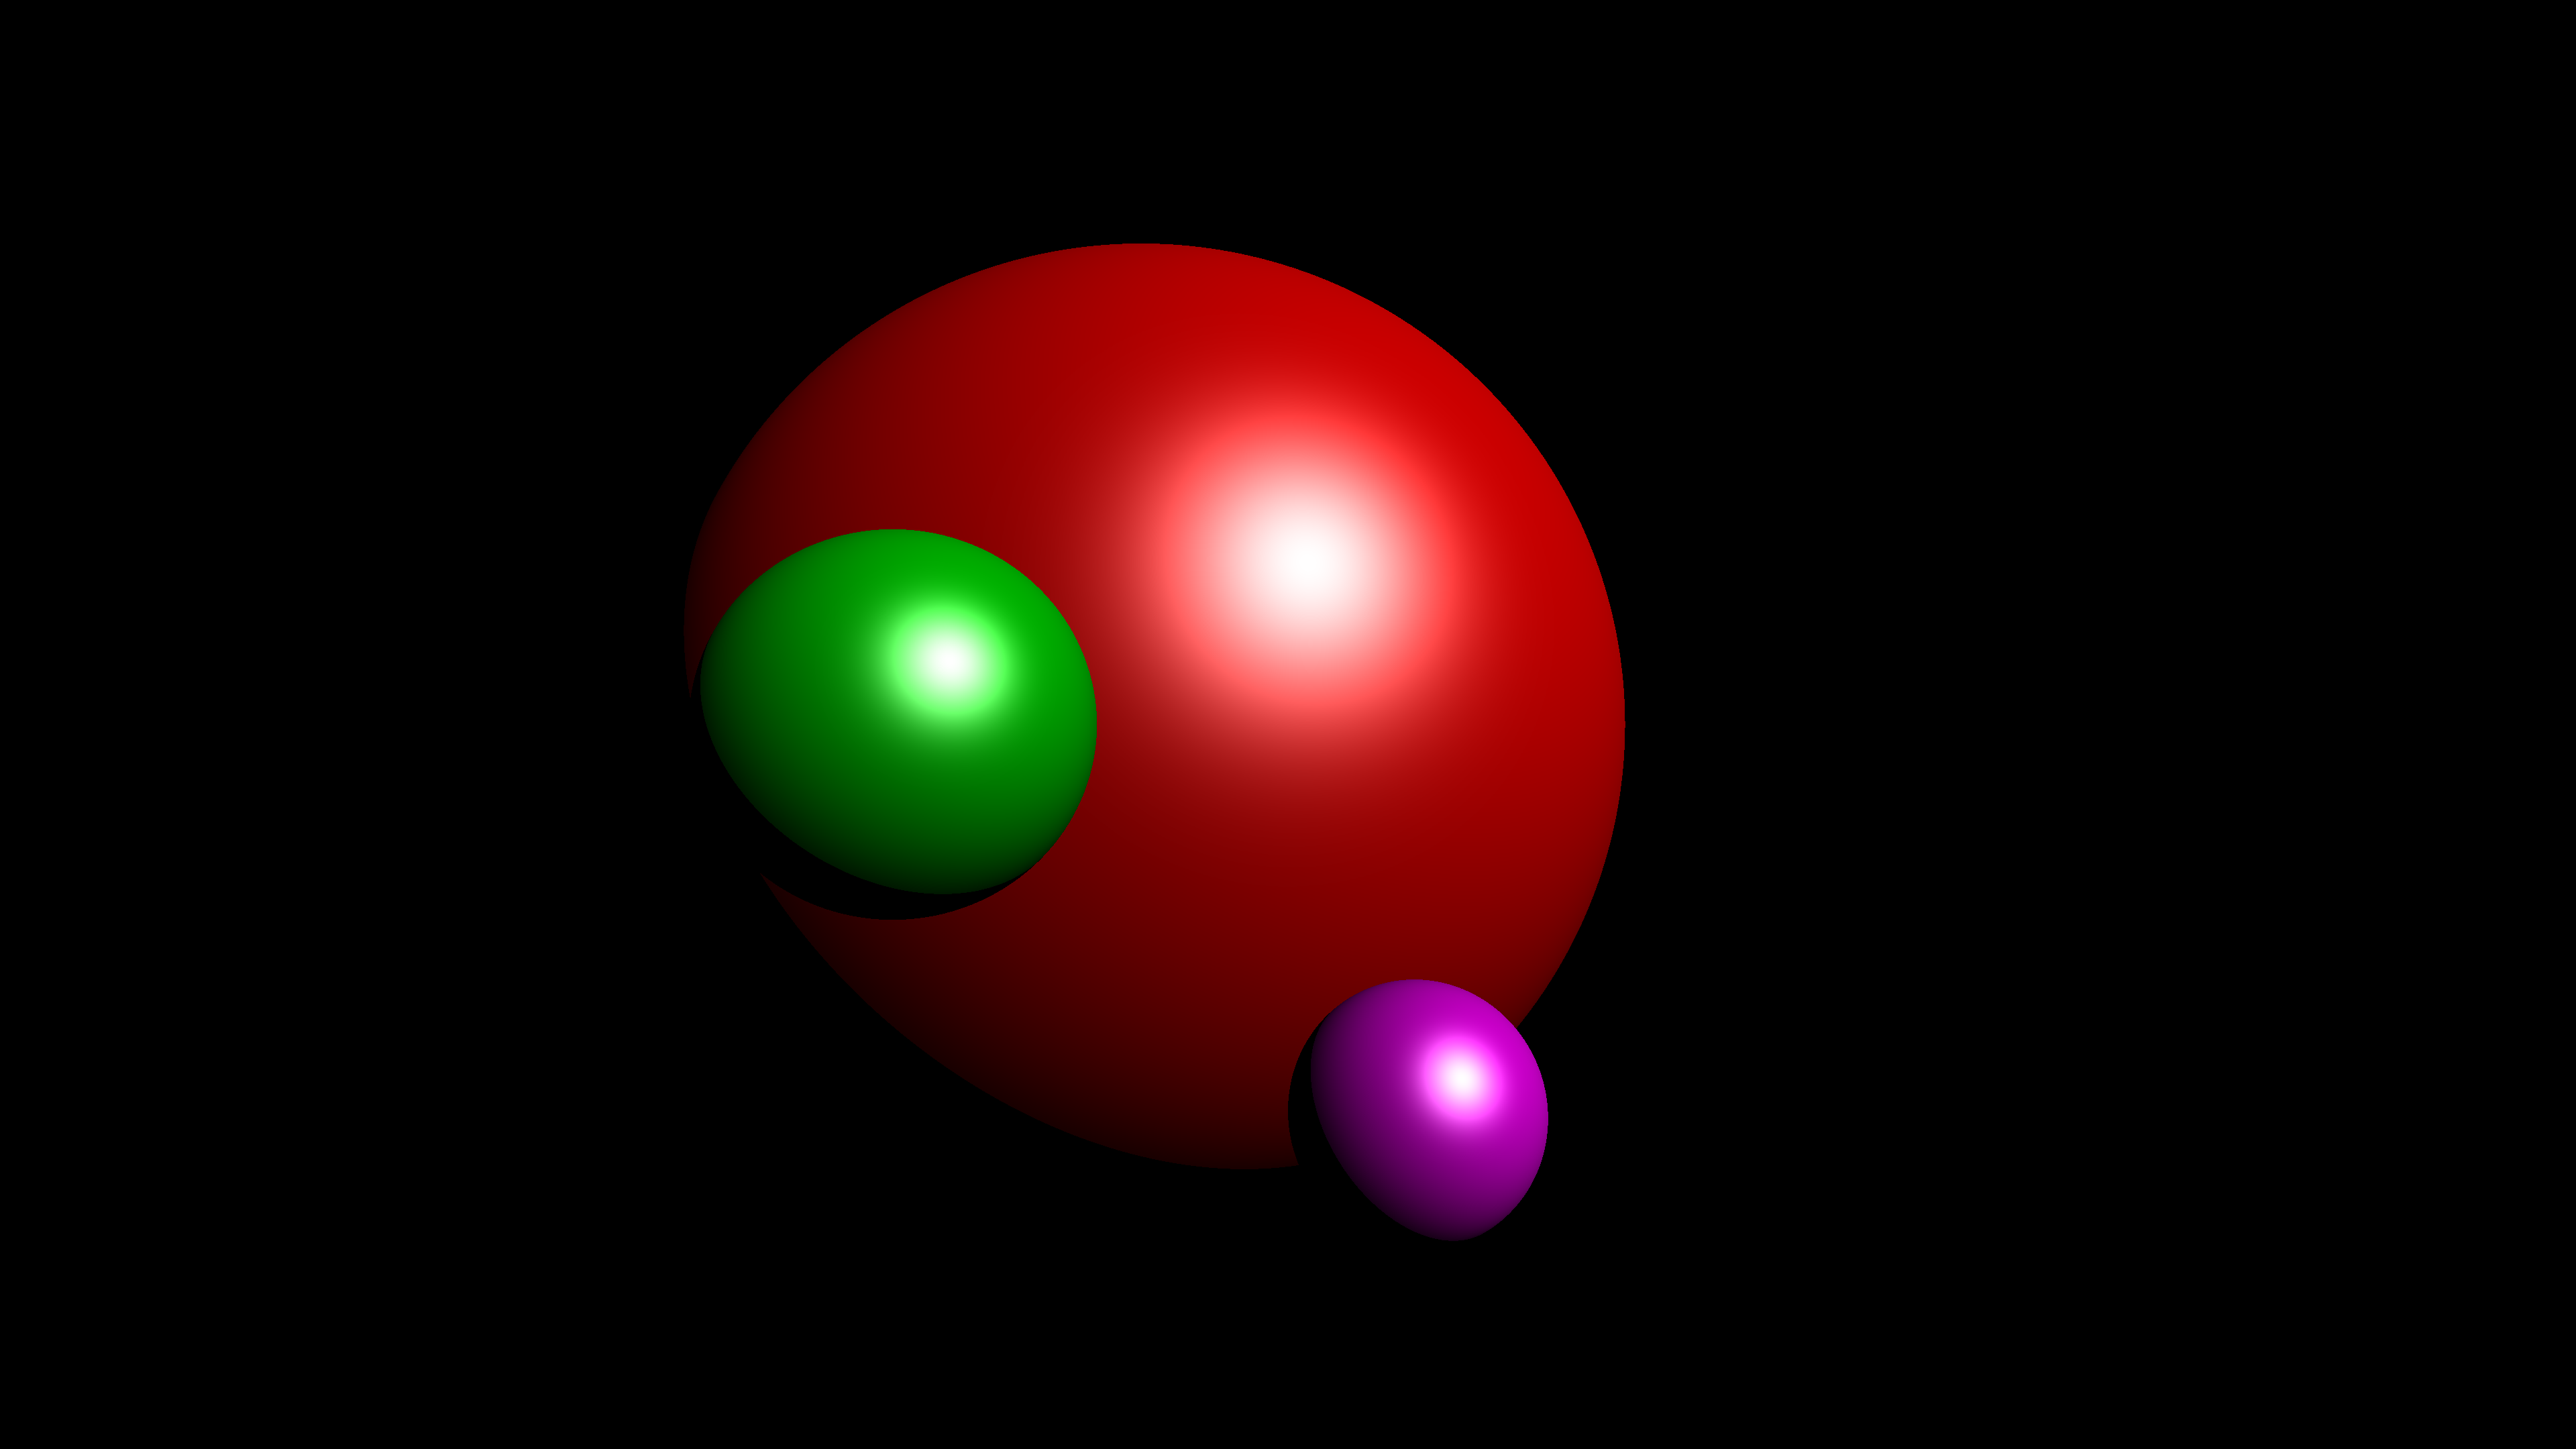
\includegraphics[width=0.7\columnwidth]{Figures/19.png}
    \caption{}
    \label{fig:figure}
\end{figure}
Vedendo il risultato, è possibile aggiungere il riflesso alle sfere e un piano.

\subsection{Finto piano}
Un finto piano può essere renderizzato utilizzando una quarta sfera, impostando un raggio quasi infinito. Questo permette di percepire la sua superficie come un piano d'appoggio.	\\
Quindi la soluzione è aggiungere alle sfere
\begin{lstlisting}[language=Python]
{ 'center': np.array([0, -9000, 0]), 'radius': 90000-0.7, 'ambient': np.array([0.1, 0.1, 0.1]), 'diffuse': np.array([0.6, 0.6, 0.6]), 'specular': np.array([1, 1, 1]), 'shininess': 100, 'reflection': 0.5 }
\end{lstlisting}

\subsection{Riflessione}
Il raggio che è renderizzato finora, parte dalla sorgente luminosa, colpisce la superficie di un oggetto e rimbalza verso la camera. Potrebbe capitare che prima di arrivare alla camera colpisca altri oggetti prima: questo è il fenomeno della riflessione. Il raggio accumula differenti colori e quando colpirà la camera si vedrà il riflesso.\\
Ogni oggetto deve avere un coefficiente di riflessione compreso tra 0 e 1. dove con 0 si indica che non riflette luce, mentre 1 è una superficie specchio. Si aggiunga tale coefficiente alle sfere:
\begin{lstlisting}[language=Python]
objects = [
    { 'center': ... , 'reflection': 0.5 },
    { 'center': ... , 'reflection': 0.5 },
    { 'center': ... , 'reflection': 0.5 },
    { 'center': ... , 'reflection': 0.5 }
]
\end{lstlisting}
Per includere la riflessione, vi è la necessità di tracciare il raggio riflesso dopo che vi è un'intersezione e di includere il contributo del colore per ogni punto di intersezione. Tale operazione va ripetuta un certo numero di volte che va definito.
\begin{figure}[H]
    \centering
    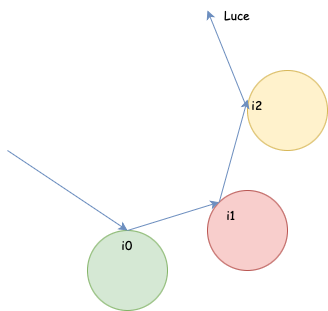
\includegraphics[width=0.7\columnwidth]{Figures/20.png}
    \caption{}
    \label{fig:figure}
\end{figure}
Per il colore di ogni pixel, bisogna sommare il contributo per ogni punto d'intersezione del raggio:
\begin{equation*}
	c_p= i_0 + r_0i_1 + r_or_1i_2+r_0r_1r_2i_3 + \dots
\end{equation*}
dove 
\begin{itemize}
	\item $c$ è il colore finale del pixel;
	\item $i$ l'illuminazione calcolata; attraverso il modello Blinn-Phong nell'$i$-esimo punto d'intersezione
	\item $r$ è la riflessione dell'$i$-esimo oggetto intersecato.
\end{itemize}
Si sceglie arbitrariamente quando fermare la somma.\\
La direzione del raggio può essere calcolata come segue:
\begin{figure}[H]
    \centering
    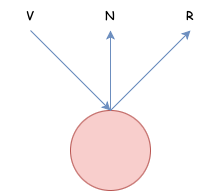
\includegraphics[width=0.7\columnwidth]{Figures/21.png}
    \caption{}
    \label{fig:figure}
\end{figure}
\begin{equation*}
	R = V - 2(V \cdot N)N
\end{equation*}
dove,
\begin{itemize}
	\item $R$ è il versore del raggio riflesso
	\item $V$ è il versore del raggio che colpisce la superficie
	\item $N$ è il versore della normale della superficie nel punto in cui viene colpita dal raggio
\end{itemize}

Si aggiunge tale funzione
\begin{lstlisting}[language=Python]
def reflected(vector, axis):
    return vector - 2 * np.dot(vector, axis) * axis
\end{lstlisting}
Il main modificato è quindi:
\begin{lstlisting}
for i, y in tqdm(enumerate(np.linspace(screen[1], screen[3], height)), position=0):
    for j, x in enumerate(np.linspace(screen[0], screen[2], width)):
        pixel = np.array([x, y, 0])
        origin = camera
        direction = normalization(pixel - origin)

        color = np.zeros((3))
        reflection = 1

        for k in range(max_depth):

            # check for intersections
            nearest_object, min_distance = nearest_intersected_object(objects, origin, direction)
            if nearest_object is None:
                break

            # compute intersection point between ray and nearest object
            intersection = origin + min_distance * direction

            normal_to_surface = normalization(intersection - nearest_object['center'])
            shifted_point = intersection + 1e-5 * normal_to_surface
            intersection_to_light = normalization(light['position'] - shifted_point)

            _, min_distance = nearest_intersected_object(objects, shifted_point, intersection_to_light)
            intersection_to_light_distance = np.linalg.norm(light['position'] - intersection)
            is_shadowed = min_distance < intersection_to_light_distance
            
            if is_shadowed:
                break

            # RGB
            illumination = np.zeros((3))

            # ambiant
            illumination += nearest_object['ambient'] * light['ambient']

            # diffuse
            illumination += nearest_object['diffuse'] * light['diffuse'] * np.dot(intersection_to_light, normal_to_surface)

            # specular
            intersection_to_camera = normalization(camera - intersection)
            H = normalization(intersection_to_light + intersection_to_camera)
            illumination += nearest_object['specular'] * light['specular'] * np.dot(normal_to_surface, H) ** (nearest_object['shininess'] / 4)

            #reflection
            color += reflection * illumination
            reflection *= nearest_object['reflection']

            #new ray origin and direction
            origin = shifted_point
            direction = reflected(direction, normal_to_surface)

        image[i, j] = np.clip(color, 0, 1)
\end{lstlisting}
\'E stata inserita la classe \texttt{tqdm} per avere più informazioni durante il processo
Eseguendo il codice completo, l'immagine di output è 
\begin{figure}[H]
    \centering
    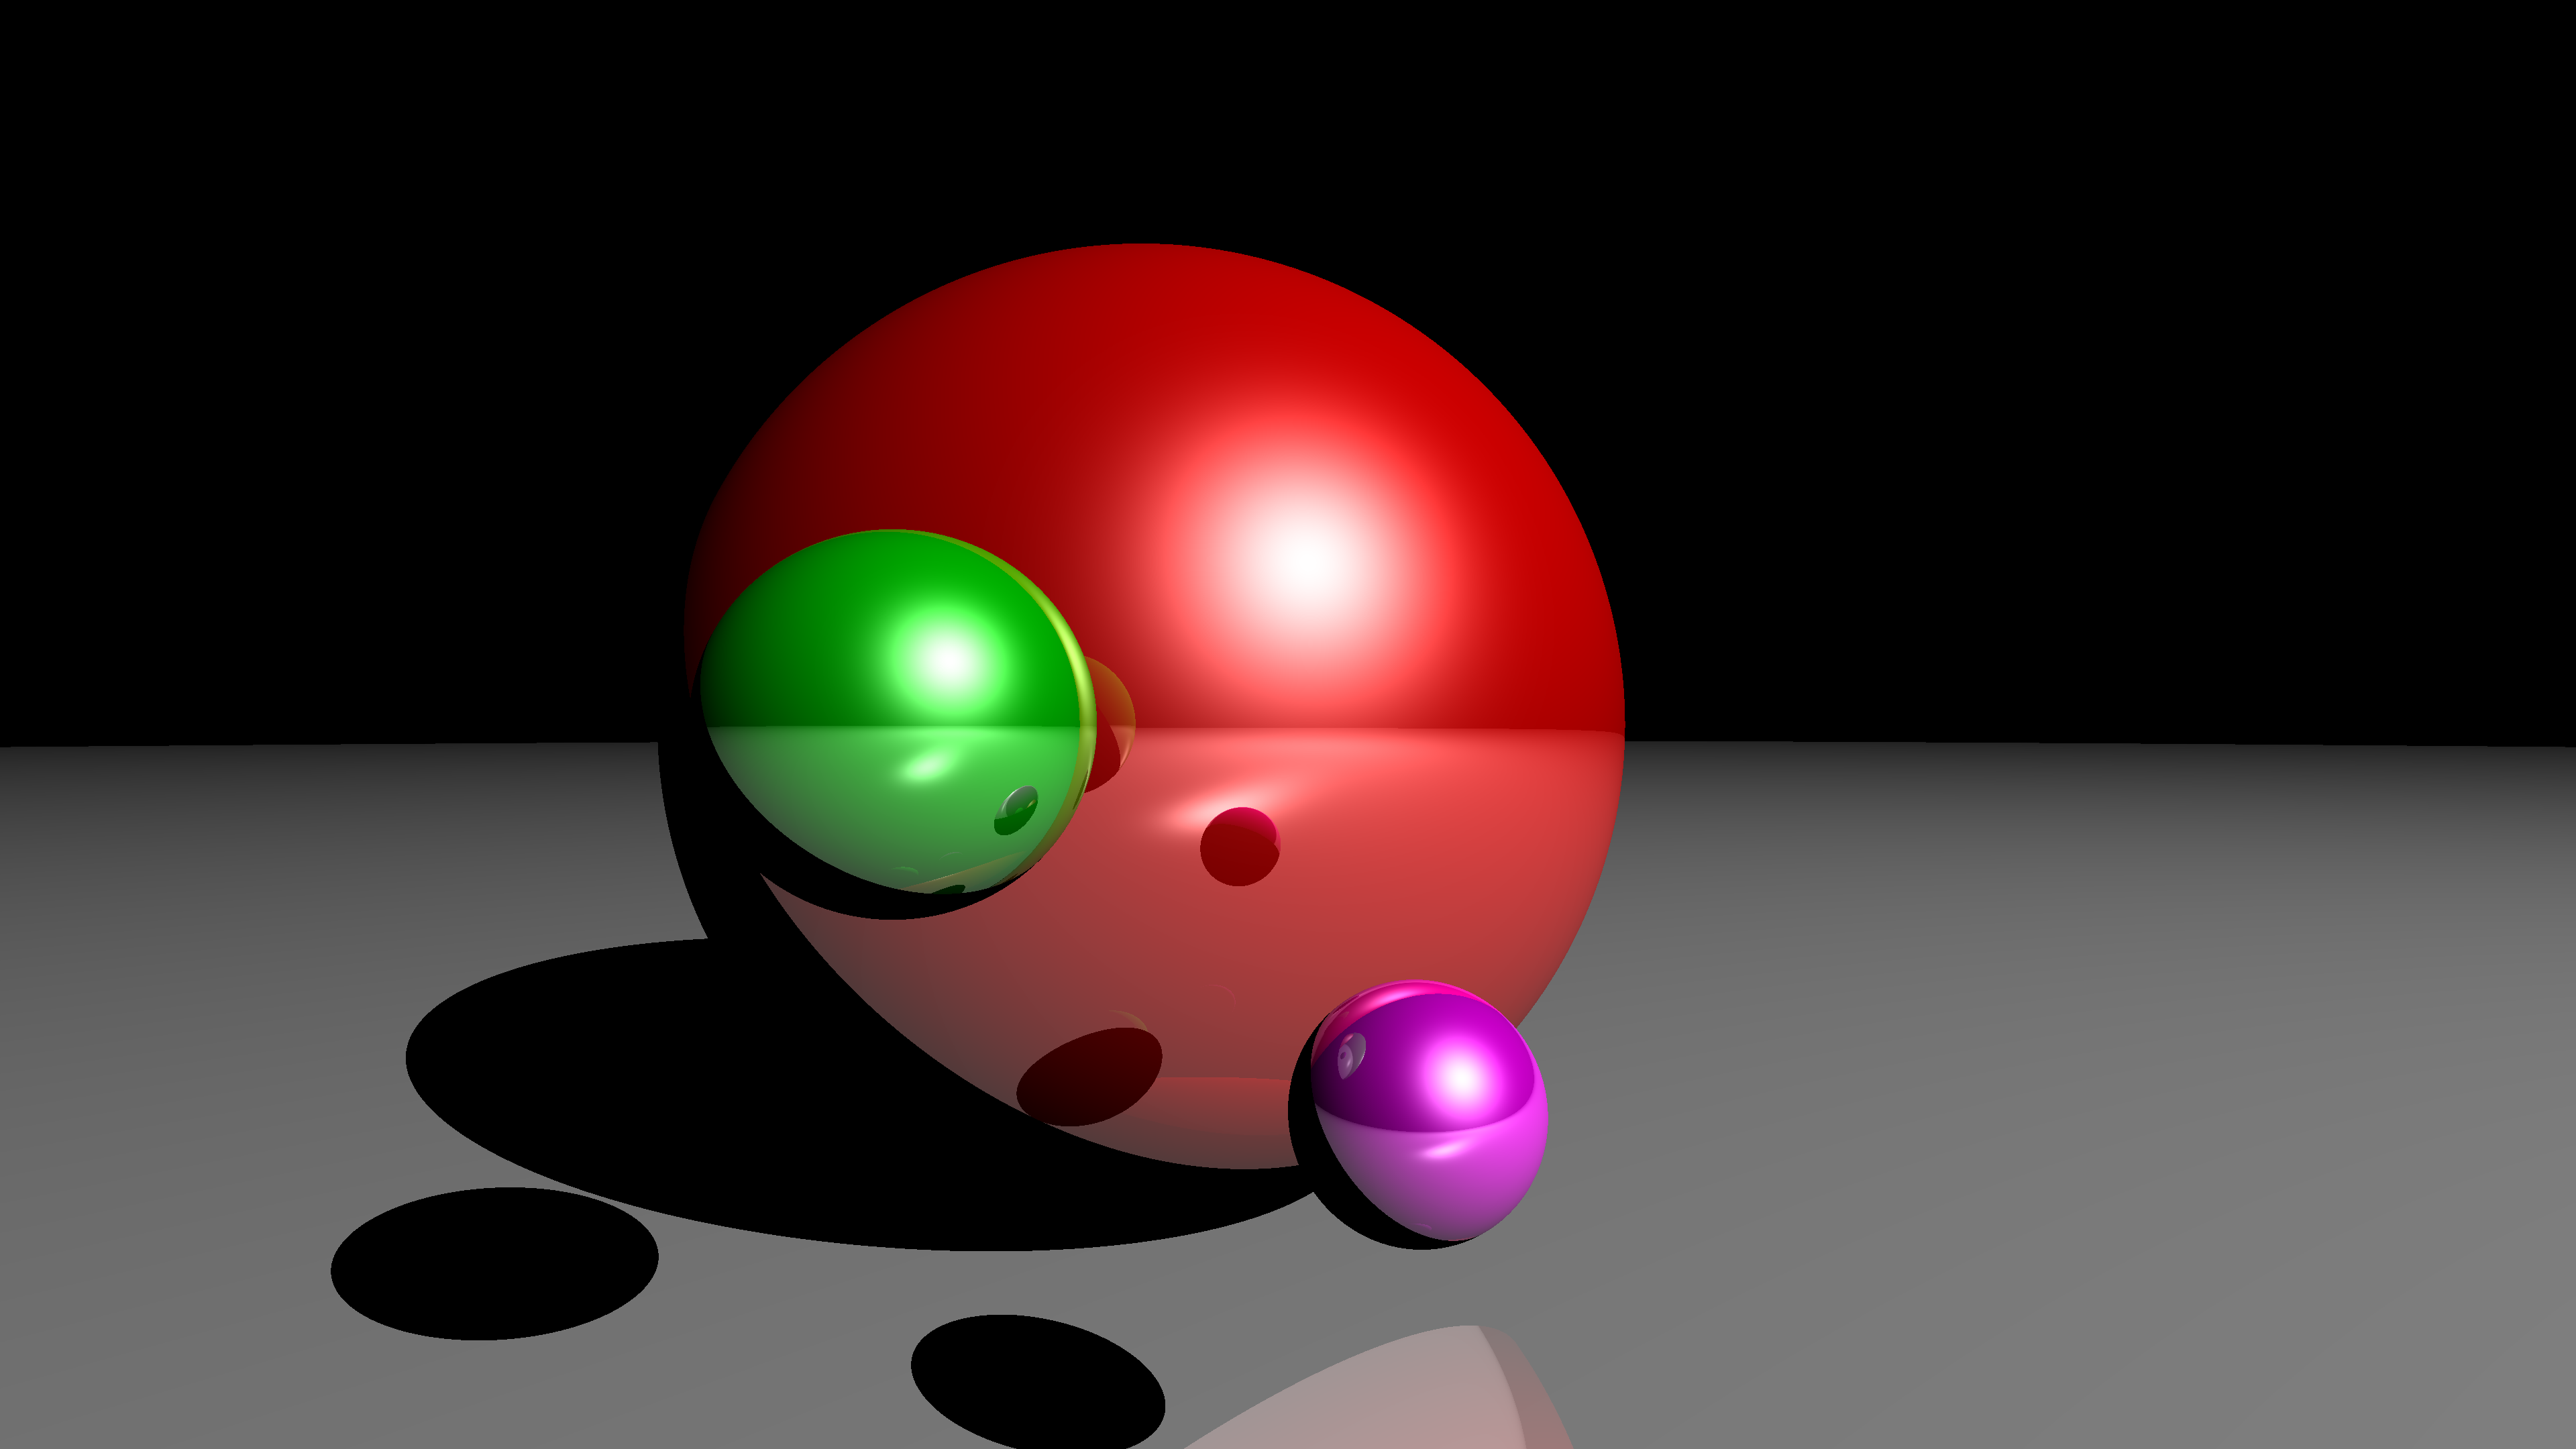
\includegraphics[width=0.7\columnwidth]{Figures/22.png}
    \caption{}
    \label{fig:figure}
\end{figure}
Il tempo impiegato per rendering è stato di $21:21$ minuti con una risoluzione $3840\times 2160$

\subsection{Generazione di un video}
Volendo generare un video, è possibile generare i diversi frame facendo variare la posizione della camera. 

					
%----------------------------------------------------------

\addcontentsline{toc}{section}{Riferimenti}
\nocite{*}
\printbibliography

%----------------------------------------------------------

\end{document}